\chapter{Evaluation}
\label{cha:evaluation}
In Chapter~\ref{cha:background}, the two most common quantum secure hash-based signature systems based on binary Merkle Trees are explained: LMS (see Section~\ref{sec:lms}) and XMSS (see Section~\ref{sec:xmss}). In Chapter~\ref{cha:methods}, the concepts \tftree (see Section~\ref{sec:dodis_t5_merkle_tree}) and \extree (see Section~\ref{sec:ext_t5_tree}) are proposed in order to speed up the common binary Merkle Tree and therefore the signature systems LMS and XMSS. 
% ! xmss not so easy possible -> bitmasks!

\section{Performance Comparison}
The general performance of the different tree concepts depending on the leaves $\ell$ is calculated with the formulas in Tables~\ref{table:general_formulas_t5_merkle}. The derivation of each formula is referenced in the column \textit{Source}.

\begin{table}
\centering
\begin{tabular}{l c c c l} 
 \hline\noalign{\smallskip}
 \multicolumn{5}{c}{\textbf{Summary: Equations Performance Calculation}} \\
\hline\noalign{\smallskip}
 & Merkle Tree & \tftree & \extree & Source  \\
 \noalign{\smallskip}
  &  & Aggr. & More Aggr. & \\
 \hline\noalign{\smallskip}
 \# hash calls keygen & $\ell-1$ & \multicolumn{2}{c}{$\frac{3}{4}(\ell-1)$} & Eq.~\ref{eq:lms_hashcalls_tree_treegen}, \ref{eq:t5_tree_gen_hashcalls} \\
% \# saved nodes (whole tree) & $2\ell-1$ & \multicolumn{2}{c}{$10\ell-1$} \\ % check if really true
% \# hash calls sign & $\emptyset$ & \multicolumn{2}{c}{$\emptyset$} & \\ % auth.path generation -> remove because not really information necessary in this table
 \# el. in auth.path & $1.44\log(\ell) $ & $1.86\log(\ell)$ & $1.74\log(\ell)$ & Eq. \ref{eq:lms_authpath_el}, \ref{eq:t5_el_authpath}, \ref{eq:ext_t5_len_authpath} \\
 \# hash calls verify & $1.44\log(\ell)$ & $1.24\log(\ell)$ & $1.12\log(\ell)$ & Eq. \ref{eq:lms_hashcalls_verify}, \ref{eq:t5_path_calc_hashcalls}, \ref{eq:ext_t5_hashcalls_verify} \\  % path calculation
 \hline
\end{tabular}
\caption{Performance of the the standard Merkle Tree (used in LMS) and \extree with the opening variants Aggressive Opening (Aggr.) and More Aggressive Opening (More Aggr.), see Sections~\ref{sec:more_aggr_opening} and \ref{sec:aggr_opening} respectively. The variable $\ell$ denotes the amount of leaves.}
\label{table:general_formulas_t5_merkle}
\end{table}

\section{NIST Parameter Set}
There exist standardized sets of values that are used for the proposed signature systems. One common example is the LMS SHA-256 parameter set proposed by the National Institute of Standards and Technology (NIST)~\cite{stateful_hashbased_sign_schemes_NIST_2020}: It is denoted in Table~\ref{table:nist_param_lms}. 
% maybe also add the one for xmss

\begin{table}
\centering
\begin{tabular}{l c c l} 
 \hline\noalign{\smallskip}
 \multicolumn{4}{c}{\textbf{NIST Parameter Set, LMS}} \\
 Parameter Set Name & Numeric Identifier & $n$ & $d$\\
 \hline\noalign{\smallskip}
 LMS\_SHA256\_M32\_H5 & 0x00000005  & 32 & 5 \\
 LMS\_SHA256\_M32\_H10 & 0x00000006  & 32 & 10 \\
 LMS\_SHA256\_M32\_H15 & 0x00000007  & 32 & 15 \\
 LMS\_SHA256\_M32\_H20 & 0x00000008  & 32 & 20 \\
 LMS\_SHA256\_M32\_H35 & 0x00000009  & 32 & 25 \\
 \hline\noalign{\smallskip}
 \end{tabular}
\caption{NIST SHA-256 parameter sets for LMS.~\cite{stateful_hashbased_sign_schemes_NIST_2020}. The variable $n$ denotes the number of bytes associated with each node in the (standard binary) Merkle tree, the parameter $d$ denotes the height of the Merkle Tree.}
\label{table:nist_param_lms}
\end{table}

\subsection{NIST Parameter Adaption}
\label{sec:nist_param_to_leaves}
% explain derivation NIST param set -> leaves
Notably, the values given in the LMS parameter set refer to the height $d$ of the Merkle Tree. When used as digital signature scheme, the leaves of the tree correspond to the amount of one-time keys. Therefore, comparing the performance of the standard Merkle Tree, \tftree and \extree based on the amount of leaves $\ell$ is the better evaluation concept than comparing the height $d$. 
The leaves $\ell$ for each tree concept are derived from $d$ in the LMS parameter set, see Table~\ref{table:nist_param_each_tree}. 

For this evaluation, we assume each leaf contains a one-time public key (i.e. there are no empty nodes). It is not possible to get the same amount of leaves for each concept, because the leaves of a perfect Merkle Tree are always a power of two, whereas the leaves of a perfect \extree always are always a  power of five. In order to still get a similar amount of leaves, the Merkle Trees with the closest power of 2 to a given power of $5^d$ is additionally used for performance evaluation with the NIST LMS parameter set: For a given $5^d$, these \textit{upper bounds} and \textit{lower bounds} are calculated by $2^{\floor{\log_2(5^d)}}$ and $2^{\ceil{\log_2(5^d)}}$ respectively. They are shown in the columns \textit{lower bound} and \textit{upper bound} in Table~\ref{table:nist_param_each_tree}.

\begin{table}
\centering
\begin{tabular}{c l l c c} 
 \hline\noalign{\smallskip}
 \multicolumn{5}{c}{\textbf{Leaves $\ell$: NIST Parameter Set, LMS}} \\
 \noalign{\smallskip} 
 & Merkle Tree & \tftree\xspace/ \extree & lower bound & upper bound \\
 $d$ & $\ell = 2^d$ & $\ell = 5^d$ & $\ell = 2^{\floor{\log_2(5^d)}}$ & $\ell = 2^{\ceil{\log_2(5^d)}}$ \\
  \hline\noalign{\smallskip}
 5 & $2^5 = 32$ & $5^5 = 3125$ & $2^{11}$ & $2^{12}$\\
 10 & $2^{10} = 1024$ & $5^{10} = 9765625$ & $2^{23}$ & $2^{24}$\\
 15 & $2^{15} = 32768$ & $5^{15} = 30517578125$ & $2^{34}$ & $2^{35}$\\ % 5^{15} 
 20 & $2^{20} = 1048576$ & $5^{20} = 95367431640625$ & $2^{46}$ & $2^{47}$\\ % 5^20 
 25 & $2^{25} = 33554432$ & $5^{25} = 298023223876953125$ & $2^{58}$ & $2^{59}$ \\ 
 \hline\noalign{\smallskip}
 \end{tabular}
\caption{Tree height $d$ out of NIST SHA-256 parameter sets for LMS (see Table~\ref{table:nist_param_lms}) converted to amount of leaves $\ell$ for for Merkle Tree, \extree. Lower bound denotes the closest power of 2 lesser than $5^d$. Upper bound denotes the closest power of 2 greater than $5^d$.}
\label{table:nist_param_each_tree}
\end{table}

\subsection{NIST Parameter Results}
After determining the parameters for each tree concept in the section before, the parameters are inserted into the equations for evaluation (see Table~\ref{table:general_formulas_t5_merkle}) to get tangible results. The performance calculation is also implemented in a Python script, see Appendix~\ref{cha:appendix2_performance_calc}.
The evaluation results for the Merkle Tree are shown in Table~\ref{table:eval_merkle_tree_NIST}, for the \tftree and \extree in Table~\ref{table:eval_t5_NIST}, for the lower/upper bound Merkle Trees in Table~\ref{table:eval_upper_lower_bound_nist}.

\begin{table}
\centering
\begin{tabular}{c l c c} 
 \hline\noalign{\smallskip}
 \multicolumn{4}{c}{\textbf{Evaluation Results NIST: Merkle Tree}} \\
 \noalign{\smallskip} 
  Leaves $\ell$ & Tree Generation & Auth.path Length & Verify \\
% $\ell$ & (in hash calls) & (in elements) & (in hash calls) \\
 \hline\noalign{\smallskip}
 $2^5$ & 31 & 5 & 5 \\
 $2^{10}$ & 1023 & 10 & 10 \\
 $2^{15}$ & 32767 & 15 & 15 \\ 
 $2^{20}$ & 1048575 & 20 & 20 \\ 
 $2^{25}$ & 33554431 & 25 & 25 \\ 
 \hline\noalign{\smallskip}
 \end{tabular}
\caption{Evaluation results for the standard Merkle Tree, given the NIST SHA-256 parameter sets as leaves $\ell$ (see Table~\ref{table:nist_param_each_tree}). The results contain the number of hash calls for tree generation and verify, as well as the length of the authentication path given the leaves $\ell$.}
\label{table:eval_merkle_tree_NIST}
\end{table}

\begin{table}
\centering
\begin{tabular}{c l c c} 
 \hline\noalign{\smallskip}
 \multicolumn{4}{c}{\textbf{Evaluation Results NIST: \tftree\xspace/ \extree}} \\
 \noalign{\smallskip} 
  Leaves & Tree Generation & Auth.path Length & Verify \\
 $\ell$ & & aggr. / more aggr. & aggr./ more aggr. \\
 \hline\noalign{\smallskip}
 $5^5$ & 2343 & 15 / 14 & 10 / 9 \\
 $5^{10}$ & 7324218 & 30 / 28 & 20 / 18 \\
 $5^{15}$ & 22888183593 & 45 / 42 & 30 / 27 \\ 
 $5^{20}$ & 71525573730468 & 60 / 56 & 40 / 36 \\ 
 $5^{25}$ & 223517417907714880 & 75 / 70 & 50 / 45 \\ 
 \hline\noalign{\smallskip}
 \end{tabular}
\caption{Evaluation results for \tftree and \extree given the NIST SHA-256 parameter sets as leaves $\ell$ (see Table~\ref{table:nist_param_each_tree}). The results contain the number of hash calls for tree generation and verify, as well as the length of the authentication path given the leaves $\ell$.}
\label{table:eval_t5_NIST}
\end{table}

\begin{table}
\centering
\begin{tabular}{c c l c c} 
 \hline\noalign{\smallskip}
 \multicolumn{5}{c}{\textbf{Evaluation Results NIST: Lower / Upper Bound Merkle Tree}} \\
 \noalign{\smallskip} 
 & lower, upper bound: $\ell$ & Tree Generation & Auth.path Length & Verify \\
 \hline\noalign{\smallskip}
 \multirow{2}{*}{$5^5$} & $\rightarrow 2^{\floor{\log_2(5^5)}} = 2^{11} $ & 2047 & 11 & 11 \\
 & $\rightarrow 2^{\ceil{\log_2(5^5)}} = 2^{12}$ & 4095 & 12 & 12 \\
 \hline\noalign{\smallskip} 
 \multirow{2}{*}{$5^{10}$} & $\rightarrow 2^{\floor{\log_2(5^10)}} = 2^{23}$ & 8388607 & 23 & 23 \\
 & $\rightarrow 2^{\ceil{\log_2(5^{10})}} = 2^{24}$ & 16777215 & 24 & 24 \\
 \hline\noalign{\smallskip} 
 \multirow{2}{*}{$5^{15}$}& $\rightarrow 2^{\floor{\log_2(5^{15})}} = 2^{34}$ & 17179869183 & 34 & 34 \\ 
 & $\rightarrow 2^{\ceil{\log_2(5^{15})}} = 2^{35}$ & 34359738367 & 35 & 35 \\ 
 \hline\noalign{\smallskip} 
 \multirow{2}{*}{$5^{20}$} & $\rightarrow 2^{\floor{\log_2(5^{20})}} = 2^{46}$ & 70368744177663 & 46 & 46 \\ 
 & $\rightarrow 2^{\ceil{\log_2(5^{20})}} = 2^{47}$ & 140737488355327 & 47 & 47 \\
 \hline\noalign{\smallskip}  
  \multirow{2}{*}{$5^{25}$} & $\rightarrow 2^{\floor{\log_2(5^{25})}} =  2^{58}$ & 288230376151711743 & 58 & 58 \\ 
 & $\rightarrow 2^{\ceil{\log_2(5^{25})}} = 2^{59}$ & 576460752303423487 & 59 & 59 \\
 \hline\noalign{\smallskip}
 \end{tabular}
\caption{Evaluation results for upper / lower bound Merkle Trees (given the NIST SHA-256 parameter sets as leaves $\ell$, see Table~\ref{table:nist_param_each_tree}). The leftmost column denotes the leaves of the \extree in between lower and upper bound Merkle Trees, see Section~\ref{sec:nist_param_to_leaves} and Table~\ref{table:nist_param_each_tree}.}
\label{table:eval_upper_lower_bound_nist}
\end{table}

The effort for tree generation for each tree concept is depicted in Figure~\ref{img:performance_tree_gen}.

\begin{figure}
\centering
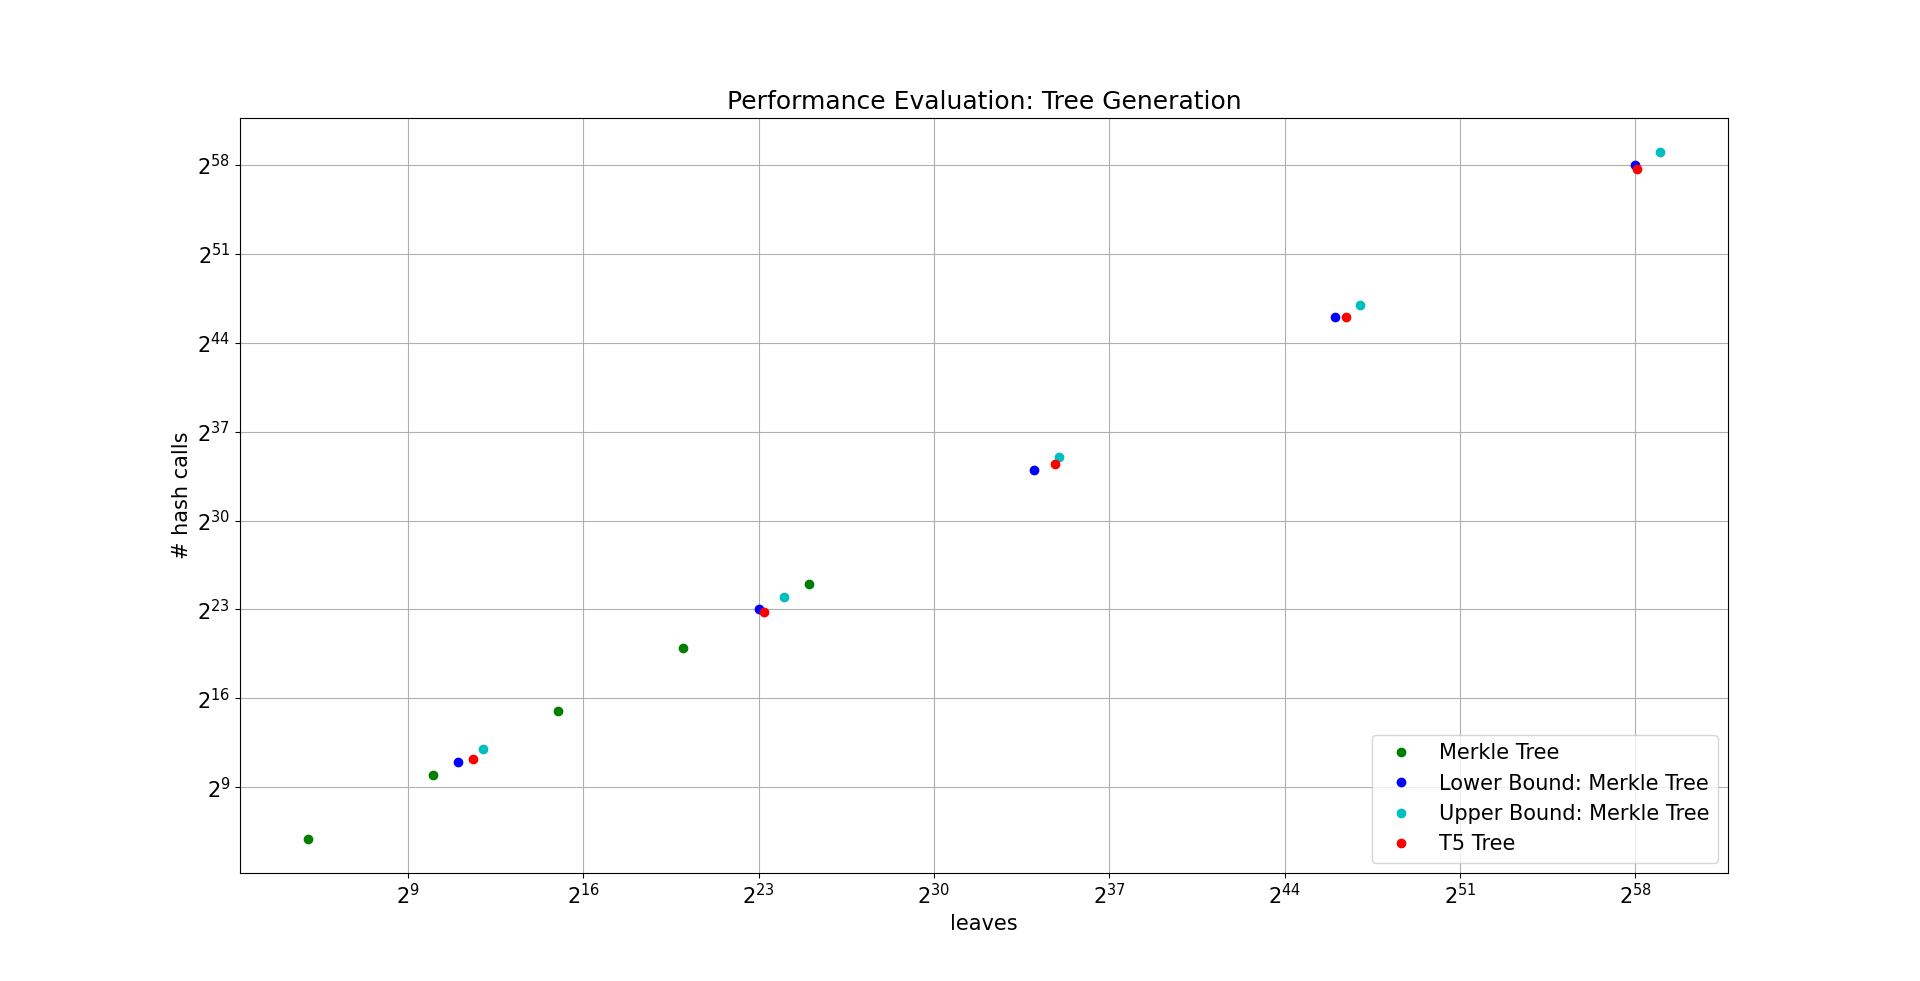
\includegraphics[width=\linewidth]{images/Evaluation/performance_tree_generation.png}
\caption{Performance of each tree concept for tree generation. The values are given in the NIST parameter set (see Table~\ref{table:nist_param_lms}), the performance equations are shown in Table~\ref{table:general_formulas_t5_merkle}.}
\label{img:performance_tree_gen}
\end{figure}

% \section{Discussion}

% \section{Future Work}
% idea for xmss, not only calculating the speedup but also concept
% concept for T5 tree when not every leaf is "filled"